\documentclass{article}
\usepackage{amsmath,fullpage,graphicx,natbib,lineno}
\title{{\tt HelioPlot}, and the treatment of \\overdispersed (U-Th-Sm)/He data}
\author{Pieter Vermeesch\footnote{School of Earth Sciences; 
Birkbeck, University of London}}
\date{}

\begin{document}
\linenumbers
\maketitle

\begin{abstract}
  More often that not, (U-Th-Sm)/He ages are overdispersed with
  respect to the formal analytical uncertainty.  The Mean Square of
  the Weighted Deviates (MSWD) is a useful tool for assessing the
  amount of overdispersion. If the MSWD is significantly greater than
  one, the ages can be parameterised by a (log)normal distribution
  with two sources of variance, which can be iteratively solved using
  the method of maximum likelihood.  The overdispersion of replicate
  (U-Th-Sm)/He ages is caused by the overdispersion of the underlying
  U-Th-Sm-He compositions, the geometric mean of which gives rise to
  the so-called `central age'.  These compositions can be normalised
  to unity and parameterised by a multivariate logistic normal
  distribution with two sources of variance, which can be iteratively
  solved by a multivariate generalisation of the aforementioned
  age-averaging algorithm.  Exact and asymmetric confidence intervals
  for the central age are obtained using a deterministic Bayesian
  algorithm.  {\tt HelioPlot} is a Java application developed for the
  purpose of plotting U-Th-(Sm)-He data on ternary diagrams and
  logratio plots that implements all these calculations.  The program
  can be downloaded from {\tt http://pvermees.andro\-pov.org/helio\-plot}.
\end{abstract}

\section{Introduction} \label{sec:intro}

Measuring several single grain U-Th-(Sm)-He aliquots per sample is not
only possible, thanks to the development of laser heating
\citep{house2000}, but also desirable, because U-Th-(Sm)-He data are
generally overdispersed with respect to the formal analytical
uncertainty and this overdispersion can only be quantified by
analysing a representative number of mineral grains. The question then
arises how to average these measurements.  Traditionally, this is done
by simply averaging the single grain age estimates, an {\it ad hoc}
solution that lacks a proper theoretical justification and does not
make full use of the data.  Potentially valuable information is lost
when the chemical composition of samples is ignored, and compositional
controls on thermochronological models may go unnoticed.  The most
natural way to study U-Th-(Sm)-He data is as a geochemical composition
on a ternary diagram or in logratio space \citep{vermeesch2008a}.\\

{\tt HelioPlot} is a data visualisation tool that plots U-Th-(Sm)-He
data on ternary diagrams and logratio plots.  The program also
calculates the so-called `central age', which is the age corresponding
to the geometric mean U-Th-(Sm)-He composition. To this end, it
applies a weighted mean algorithm taking into account both the
analytical uncertainty and any possible overdispersion simultaneously,
in contrast with \citet{vermeesch2008a}'s web calculator, which
propagated them separately. U-Th-(Sm)-He data are often overdispersed
with respect to the analytical uncertainty, for reasons that have been
discussed elsewhere \citep{fitzgerald2006, shuster2006}. The amount of
overdispersion can be quantified using the Mean Square of the Weighted
Deviates \citep[MSWD, ][]{mcintyre1966}.  Given a dataset of n age
measurements, or the logarithms thereof (t$_i$, for 1$\leq$i$\leq$n),
the MSWD is a measure of the ratio of the observed scatter of the data
points (t$_i$) around the mean value ($\bar{t}$) to the expected
scatter from the assigned errors ($\sigma_i$):

\begin{equation}
MSWD = \frac{1}{n-1} \sum_{i=1}^n \frac{(t_i - \bar{t})^2}{\sigma_i^2}
\label{eq:MSWDt}
\end{equation}

If the assigned errors are the only cause of scatter, the MSWD will
tend to be near unity.  MSWD values much less than unity indicate
either overestimated analytical errors or unrecognized
error-correlations.  MSWD values much greater than unity generally
indicate either underestimated analytical errors, or the presence of
non-analytical scatter. {\tt HelioPlot} implements methods to deal
with the latter situation.\\

Although there is no formally agreed convention for calculating the
average of multiple (U-Th)/He ages, this is either done by computing
the unweighted arithmetic mean, ignoring the analytical precision, or
by calculating the error-weighted mean, ignoring overdispersion.
Section~\ref{sec:ages} introduces a one-dimensional weighted mean
algorithm that deals with analytical precision and overdispersion
simultaneously, using the method of maximum likelihood.
Section~\ref{sec:compositions} generalises this method to
compositional data space, so as to calculate the best estimate for the
central age, taking into account both the internal and external
reproducibilities of the data, as well as their full covariance
structure.  `Conventional' propagation of uncertainty for the central
age, as implemented by \citet{vermeesch2008a}, involves linearisation
by a first-order Maclaurin series expansion, which may be inaccurate.
Section \ref{sec:ci} proposes a deterministic algorithm to avoid this
problem, yielding exact confidence intervals for the central age.
Finally, Section \ref{sec:helioplot} provides further details about
{\tt HelioPlot} and illustrates its usefulness with a number of real
world examples.

\section{Overdispersed ages} \label{sec:ages}

Assume that the ages (or the logarithm of the ages) come from a normal
distribution of the form

\begin{equation}
  \label{eq:norm1}
  t_i \sim N(\mu,\sigma_i^2 + \xi^2)
\end{equation}

where $\mu$ denotes the mean and $\xi^2$ is the amount of {\it
  overdispersion}, i.e. the excess scatter that cannot be explained by
the analytical uncertainty alone. Unbiased estimates $\hat{\mu}$ and
$\hat{\xi}^2$ for these two parameters can be obtained by maximising the
likelihood l:

\begin{equation}
l \equiv \prod_{i=1}^n 
\frac{exp\left(-\frac{(t_i - \hat{\mu})^2}
{2(\sigma_i^2 + \hat{\xi^2_i})}\right)}
{\sqrt{2\pi(\sigma_i^2 + \hat{\xi}^2)}}
  \label{eq:l1}
\end{equation}

\noindent or, more conveniently, the log-likelihood L $\equiv$ log(l):

\begin{equation}
L = - \frac{1}{2} \sum_{i=1}^n 
\left[
\frac{(t_i - \hat{\mu})^2}{\sigma_i^2+\hat{\xi}^2}
+ ln(\sigma_i^2 + \hat{\xi}^2) + ln(2\pi)
\right]
  \label{eq:L1}
\end{equation}

\noindent Calculating the derivatives of L with respect to $\hat{\mu}$ and
$\hat{\xi}^2$ and setting them to zero to find the maximum likelihood:

\begin{align}
& \frac{\partial L}{\partial \hat{\mu}}  = 
\sum_{i=1}^n \frac{t_i - \hat{\mu}}{\sigma_i^2 + \hat{\xi}^2} = 0
\label{eq:Lmu1}\\
&\frac{\partial L}{\partial \hat{\xi}^2}  =
\sum_{i=1}^n \left[ \frac{(t_i-\hat{\mu})^2}{(\sigma_i^2+\hat{\xi}^2)^2}
- \frac{1}{\sigma_i^2+\hat{\xi}^2} \right] = 0 
\label{eq:Lxi1}
\end{align}

which can be solved iteratively for $\hat{\mu}$ and $\hat{\xi}^2$.  The
variance $\hat{\sigma}_{\mu}^2$ of the weighted mean $\hat{\mu}$ is given by
the inverse of the Fisher Information, i.e.  the negative expected
value of the second derivative of the log-likelihood function with respect
to $\hat{\mu}$:

\begin{equation}
\hat{\sigma}_{\mu}^2
=
\frac{1}{
\sum_{i=1}^n 1 / (\sigma_i^2 + \hat{\xi}^2)
}
\label{eq:sigma1}
\end{equation}

\section{Overdispersed compositions}
\label{sec:compositions}

U, Th and He form a ternary system, can be plotted on a ternary
diagram, and are subject to the peculiar mathematics of the ternary
dataspace. The `central age' is calculated from the geometric mean
composition of a U-Th-(Sm)-He dataset and is a more accurate estimator
of the true age than the arithmetic mean \citep{vermeesch2008a}.  This
concept can be easily generalised to four dimensions and this section
will, therefore, discuss the case of (U-Th-Sm)/He dating.  Given n
single grain measurements [U$^i$, Th$^i$, Sm$^i$, He$^i$]
(1$\leq$i$\leq$n), the calculation of a central age involves a
bijection from the four-dimensional `simplex' to a three-dimensional
Euclidean logratio-space \citep{aitchison1986, vermeesch2008a}:

\begin{equation}
  \label{eq:logratio-transform}
  v^i  =  ln\left(\frac{[U^i]}{[He^i]}\right),~
  w^i  =  ln\left(\frac{[Th^i]}{[He^i]}\right),~
  x^i  =  ln\left(\frac{[Sm^i]}{[He^i]}\right)
\end{equation}

The central age is obtained by calculating the average logratio
composition ($\overline{v}$, $\overline{w}$, $\overline{x}$) and
converting it to a geometric mean composition using the inverse
logratio transformation:

\begin{equation}
  \label{eq:inverse-transform}
\begin{split}
&  \overline{U}  =  \frac{e^{\overline{v}}}{e^{\overline{v}}+e^{\overline{w}}+e^{\overline{x}}+1},~
  \overline{Th}  =  \frac{e^{\overline{w}}}{e^{\overline{v}}+e^{\overline{w}}+e^{\overline{x}}+1}\\
&  \overline{Sm}  =  \frac{e^{\overline{x}}}{e^{\overline{v}}+e^{\overline{w}}+e^{\overline{x}}+1},~
  \overline{He}  =  \frac{1}{e^{\overline{v}}+e^{\overline{w}}+e^{\overline{x}}+1}
\end{split}
\end{equation}

This result is then plugged into the U-Th-(Sm)-He age equation.  
\\

The problem of averaging the compositions is very similar to the
problem of averaging the ages discussed in the previous section.
Given n logratio measurements X$^i$ and their (co)variances $E^i$ (1
$\leq$ i $\leq$ n):

\begin{equation}
X^i \equiv
\Biggl[
\begin{array}{c}
v^i\\
w^i\\
x^i
\end{array}
\Biggr]
\mbox{~and~}
E^i \equiv
\Biggl[
\begin{array}{ccc}
\sigma_{v^i}^{2} & cov_{v^i,w^i} & cov_{v^i,x^i} \\
cov_{v^i,w^i} & \sigma_{w^i}^{2} & cov_{w^i,x^i} \\
cov_{v^i,x^i} & cov_{w^i,x^i} & \sigma_{x^i}^{2}
\end{array}
\Biggr]
\label{eq:Ai}
\end{equation}

\noindent our  aim is to  develop an  algorithm to  calculate the  weighted mean
M and its covariance matrix $\Sigma$:

\begin{equation}
M \equiv
\Biggl[
\begin{array}{c}
\overline{v}\\
\overline{w}\\
\overline{x}
\end{array}
\Biggr]
\mbox{~and~}
\Sigma \equiv
\Biggl[
\begin{array}{ccc}
\sigma^2_{\overline{v}}      & cov_{\overline{v},\overline{w}}   & cov_{\overline{v},\overline{x}}\\
cov_{\overline{v},\overline{w}}  & \sigma^2_{\overline{w}}       & cov_{\overline{w},\overline{x}}\\
cov_{\overline{v},\overline{x}}  & cov_{\overline{w},\overline{x}}   & \sigma^2_{\overline{x}}\\
\end{array}
\Biggr]
\label{eq:Abar}
\end{equation}

In principle, the logratio covariances (E$^i$) could be directly
determined from the raw mass spectrometer measurements. In practice,
however, they are calculated from the individual concentrations by
linear approximation, using Equation 21 of \citet{vermeesch2008a},
which assumes that the errors on the individual concentrations are
Normal and independently distributed.  Rather than propagating the
internal and external uncertainties separately, as done by
\citet{vermeesch2008a}, this section introduces a weighted mean
algorithm that considers both factors simultaneously, using a
multivariate generalisation of the one-dimensional maximum likelihood
algorithm developed in Section \ref{sec:ages}. First, redefine the
MSWD in matrix form:

\begin{equation}
MSWD = \frac{1}{df} \sum_{i=1}^n 
(X^i-M)'[E^i]^{-1}(X^i-M)
\label{eq:MSWDc}
\end{equation}

\noindent where df = d $\times$ (n - 1) is the number of degrees of freedom of
the problem, with d = 2 for (U-Th)/He and d = 3 for (U-Th-Sm)/He
dating. Note that, because the variability of Sm does not contribute
as much to the age dispersion as that of U and Th, it is better to use
only the latter two elements for the MSWD calculation. If MSWD $\gg$
1, the data are overdispersed and, in analogy with Equation
\ref{eq:norm1}, we will assume that the observations come from a
multivariate normal distribution of the form

\begin{equation}
X^i \sim N(M, E^i + \Xi)
\label{eq:norm2}
\end{equation}

\noindent where M denotes the mean and $\Xi$ is the overdispersion. 
The log-likelihood is given by:

\begin{equation}
L = - \frac{1}{2} \sum_{i=1}^n 
\left(
(X^i-\hat{M})'[E^i + \hat{\Xi}]^{-1}(X^i-\hat{M})
+ ln|E^i + \hat{\Xi}| + 3~ln(2\pi)
\right)
  \label{eq:L2}
\end{equation}

\noindent $\hat{M}$ and $\hat{\Xi}$ can be found by solving the following
system of non-linear equations:

\begin{align}
& \frac{\partial L}{\partial \hat{M}}  = 
\sum_{i=1}^n [(E^i+\hat{\Xi})^{-1}(X^i-\hat{M})] = 0
\label{eq:Lmu}\\
&\frac{\partial L}{\partial \hat{\Xi}}  =
\sum_{i=1}^n [(E^i+\hat{\Xi})^{-1}(X^i-\hat{M})(X^i-\hat{M})'(E^i+\hat{\Xi})^{-1}
- (E^i+\hat{\Xi})^{-1}] = 0 
\label{eq:Lxi}
\end{align}

The covariance matrix $\hat{\Sigma}$ of the weighted mean $\hat{M}$ is
obtained by inverting the Fisher Information matrix, i.e.  the matrix
of the negative expected values of the second derivatives of the
log-likelihood function:

\begin{equation}
\hat{\Sigma}
=
\Biggl[
\sum_{i=1}^n (E^i+\hat{\Xi})^{-1}
\Biggr]^{-1}
\label{eq:Sigma}
\end{equation}

\section{Confidence intervals} \label{sec:ci}

Using the covariance matrix of the logratio average ($\hat{\Sigma}$),
and performing a linear error propagation, it is straightforward to
calculate the covariance matrix of the geometric mean composition
($\hat{\Gamma}$), evaluated at $\hat{M}$:

\begin{equation}
\label{eq:gamma}
\hat{\Gamma} = A'\hat{\Sigma} A
\end{equation}

where A is the matrix of first derivatives of Equation \ref{eq:inverse-transform}:

\begin{equation}
\label{eq:df}
A =  \Biggl[
\begin{array}{cccc}
\frac{\partial U}{\partial v} & \frac{\partial Th}{\partial v} & 
\frac{\partial Sm}{\partial v} & \frac{\partial He}{\partial v}\\
\frac{\partial U}{\partial w} & \frac{\partial Th}{\partial w} & 
\frac{\partial Sm}{\partial w} & \frac{\partial He}{\partial w}\\
\frac{\partial U}{\partial x} & \frac{\partial Th}{\partial x} & 
\frac{\partial Sm}{\partial x} & \frac{\partial He}{\partial x}\\
\end{array}
\Biggr]_{\hat{M}}
\end{equation}

Equation \ref{eq:gamma} contains an expression for the covariances of
the geometric mean composition, which were omitted by
\citet{vermeesch2008a} but are required for a full propagation of age
uncertainty. However, even the complete error propagation may be
inaccurate because it is based on a first order Maclaurin series
expansion of Equation \ref{eq:inverse-transform}, which is highly
non-linear.  This problem can be circumvented using numerical
techniques, such as the following deterministic algorithm.  First,
build a regular grid across the two (for U-Th-He) or three (for
U-Th-Sm-He) dimensions of logratio space (Figure \ref{fig:ci}.a).
Second, for each of these grid points, calculate (a) its likelihood
under a normal distribution with mean $\hat{M}$ and covariance matrix
$\hat{\sigma}$, and (b) the corresponding age.  Third, calculate the
Bayesian cumulative posterior distribution by ranking the numerical
data in order of increasing age and computing the running sum of the
likelihoods.  Fourth, obtain an asymmetrical 95\% confidence interval
from the 2.5 and 97.5 percentiles of the posterior distribution
(Figure \ref{fig:ci}.b).

\section{Applications} \label{sec:helioplot}

{\tt HelioPlot} is a computer program for visualising U-Th-(Sm)-He
data on ternary diagrams and logratio plots that implements all the
above calculations, including the computation of central ages and 95\%
confidence intervals.  Equations \ref{eq:Lxi1} and \ref{eq:Lxi} are
solved using Newton's method.  {\tt HelioPlot} was written in Java and
is, therefore, perfectly platform independent.  The program and its
source code can be downloaded free of charge from {\tt
  http://pvermees.andro\-pov.org/helio\-plot}.  Data can be copied
and pasted to-and-from Microsoft Excel, or entered directly using the
built-in editing tools.  Data files are saved in a
comma-separated-variable ({\tt .csv}) format. Samarium is an optional
input parameter and the complete functionality of the program is still
available when Sm is missing. If Sm is absent, it will be assumed to
be zero, and the data naturally reduce to their two dimensions in
compositional datapace.  If Sm is present, the geometric mean Sm
composition is used as a common reference for the ternary diagrams and
logratio plots.  Colour is used to visualise the Sm content of
aliquots, or any other numerical quantity, such as sample number
(Figure \ref{fig:helioplot}.a), grain size (Figure
\ref{fig:helioplot}.b), elevation, or, for the case of double-dated
grains, a U-Pb or fission track age \citep{campbell2005}.  {\tt
  HelioPlot} is capable of saving the graphical output as either
bitmap or vector images, in a {\tt .png} or {\tt .pdf} format,
respectively.
\\

Example input files are provided on the website for testing purposes.
Figure \ref{fig:helioplot}.b shows the output for one of these files,
based on a published (U-Th)/He dataset \citep{vermeesch2007b}, which
was $\alpha$-ejection corrected according to the guidelines of
\citet{ketcham2009}. The output includes the arithmetic and geometric
mean ages and their standard errors, calculated using the methods of
Section \ref{sec:ages}, in addition to the central age, its standard
error and 95\% confidence interval, calculated according to the
algorithm of Section \ref{sec:compositions}.  Three separate MSWDs are
given, reflecting the overdispersion of the ages and the U-Th-He
compositions.

\section{Conclusions}

The aim of this paper was to bring the statistical treatment of
U-Th-(Sm)-He data on an equal footing with more established
geochronometers such as U-Pb, $^{40}$Ar/$^{39}$Ar, or fission tracks.
Weighted least squares algorithms similar to the maximum likelihood
methods of Sections \ref{sec:ages} and \ref{sec:compositions} have
been used in U-Pb \citep{ludwig1998} and fission track dating
\citep{galbraith1990b}.  Visual aids such as the U-Pb concordia
diagram, the Rb-Sr isochron, or the fission track radial plot can be
very useful for the exploratory analysis of geochronological data. The
ternary diagram and logratio plot play the same role for helium
thermochronology, as they bring out the full information content of
U-Th-(Sm)-He data, and can help to reveal patterns between aliquots
and samples that may not be seen otherwise.

\section*{Acknowledgments}

John Rudge formulated equation \ref{eq:norm2}, from which the rest of
the calculations followed naturally. He and an anonymous reviewer are
gratefully acknowledged for this and other constructive comments.

\bibliography{/home/pieter/Documents/biblio}
\bibliographystyle{/home/pieter/Documents/elsart-harv}

\section*{Figures}

\begin{figure}[h]
a.\includegraphics[width=.5\textwidth]{Bayes2.pdf}
b.\includegraphics[width=.45\textwidth]{CI2.pdf}
\caption{a. the deterministic Bayesian algorithm collects a large
  number of ages across a regular grid in logratio space (crosses),
  and records the corresponding logistic normal likelihood of the data
  (ellipse); b.  95\% confidence intervals are then simply calculated
  by looking up the 2.5 and 97.5 percentiles of the resulting
  `posterior distribution'.}
\label{fig:ci}
\end{figure}

\begin{figure}[h]
a.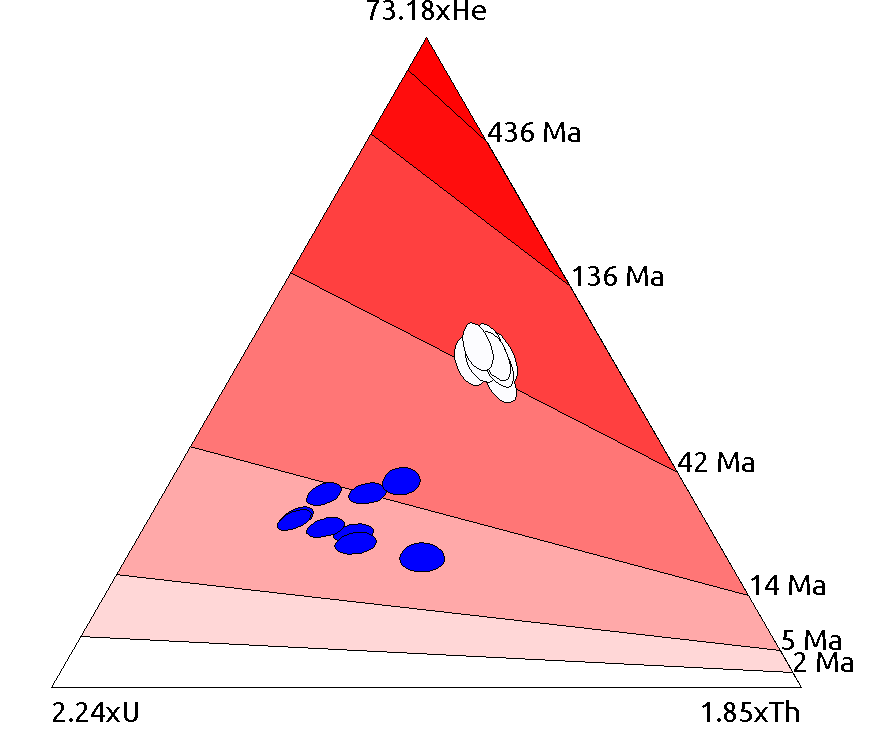
\includegraphics[width=.45\textwidth]{ternaryplot.pdf}
b.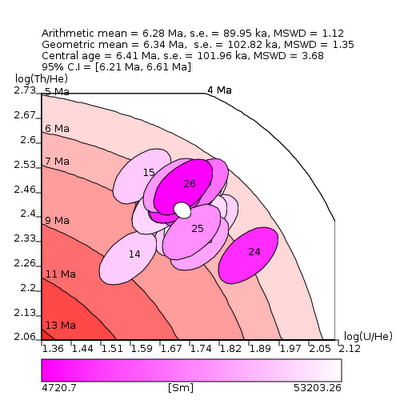
\includegraphics[width=.45\textwidth]{logratioplot.pdf}
\caption{Two diagrams produced by {\tt HelioPlot}. (a) Ternary diagram
  with two synthetic U-Th-He samples ($U* = \frac{U-0.0611}{0.362}$,
  $Th* = \frac{Th-0.574}{0.362}$, $He* = \frac{He-0.0041}{0.362}$).
  (b) Logratio plot of U-Th-He data from Naxos \citep{vermeesch2007b},
  colour-coded according to grain size.  The geometric mean
  composition is shown as a white ellipse.}
\label{fig:helioplot}
\end{figure}

\end{document}
